\chapter{Input and output}

A number of years ago, Jeannette Wing published a terrific editorial with the title {\it Computational Thinking}, or in her own words, ``Ways to Think Like a Computer Scientist'' (see Communications of the ACM, March 2006).
This 3-page article summarizes many of the problem-solving techniques you will discover while learning to program.
Everyone interested in learning computer science beyond programming should read it.
She defines the field this way:

\index{computer science}

\begin{quote}
{\bf ``Computer science is the study of computation---what can be computed and how to compute it.''}
\end{quote}

So far the only programs we've looked at simply display messages, which doesn't involve a lot of real computation.
But that will change quickly as we begin to work with more types of data.
This chapter will show you how to read input from the keyboard, use that input to calculate a result, and then format that result for output.
We will also look at some technical details about how operating systems work.


\section{Java class library}

\index{library}

Like most programming languages, Java has an extensive {\bf library} of class and method definitions that you can use in your programs.
You can browse this library on Oracle's website:
\url{http://docs.oracle.com/javase/7/docs/api/}

\index{package}

The standard edition of Java comes with {\em several thousand} classes, which can be both exciting and intimidating.
To help keep things organized, classes are grouped into {\bf packages}.
Just as each class is a separate file, each package is a separate folder.

\begin{figure}[!h]
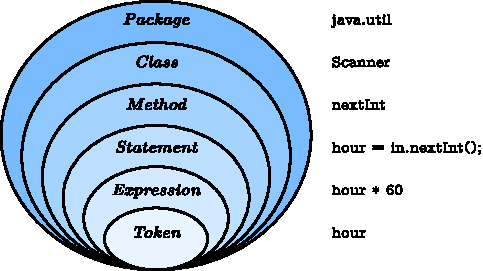
\includegraphics[width=4in]{package.pdf}
\caption{Elements of the Java language, from largest to smallest.}
\end{figure}

Two library classes we have seen thus far, \java{System} and \java{String}, belong to the \java{java.lang} package.
According to the documentation, \java{java.lang} ``provides classes that are fundamental to the design of the Java programming language.''
Note there is a major difference between the Java {\em language}, which deals with syntax and grammar, and the Java {\em library}, which provides the built-in classes.
In fact, most of the Java library itself is written in Java!

\index{import}
\index{statement!import}

In order to use a class defined in another package (and in another folder), you have to {\bf import} it first:

\begin{code}
import java.io.File;
import java.io.PrintStream;
import java.util.Date;
import java.util.Scanner;
\end{code}

All \java{import} statements appear at the beginning of the source file, above the class definition.
It's not uncommon for Java programs to have dozens of import statements.
Because they are so fundamental, all classes in \java{java.lang} are imported automatically.
That is why we haven't needed the \java{import} statement until now.


\section{The System class}
\label{system}

\index{System class}
\index{class!System}
\index{object}

When you call \java{System.out.println}, you are referring to the \java{out} variable declared in the \java{System} class.
The \java{out} variable's type is \java{PrintStream}, which provides methods for ``printing'' data.
Both \java{System} and \java{PrintStream} are written in Java, and later in the book we'll examine their source code.
For now, you should understand that \java{System.out} is an {\bf object} of type \java{PrintStream}.
Because Java is an {\em object-oriented} language, much of the library is organized around objects that perform specific actions.

\begin{figure}[!h]
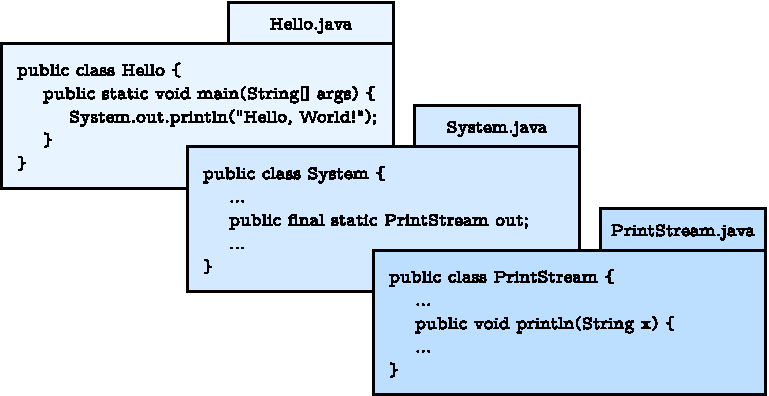
\includegraphics{system.pdf}
\caption{\java{System.out.println} references the \java{out} variable of the \java{System} class,
\\ which has the type \java{PrintStream}, which has a method called \java{println}.}
\end{figure}

\index{operating system}

As with most software, Java programs run on top of an {\bf operating system} that manages the keyboard, the display, main memory, disk drives, printers, the network, and other hardware resources.
Common examples of operating systems include Android, iOS, Linux, Mac OS~X, and Windows.
When starting Java programs, the operating system directs \java{System.out} to the screen.

\java{System.out} can display the value of any type of variable.
Indeed, you can even use \java{System.out} to print the value of \java{System.out}:

\begin{code}
System.out.println(System.out);
\end{code}

The result is:

\begin{stdout}
java.io.PrintStream@685d72cd
\end{stdout}

\index{address}

When Java prints an object, it prints the type of the object (\java{PrintStream}), the package where the type is defined (\java{java.io}), and the {\bf address} or location of the object in memory (after the \java{@} sign).
In this example the address is \java{685d72cd}, but if you run the same code you will likely get something different.
You can think of the address as a unique identifier for the object.

\index{abstraction}

Note the exact type of display doesn't matter, whether it's a 5-inch touch screen or 30-inch monitor.
From the programmer's point of view, \java{System.out} simply provides the means for printing messages.
Computer scientists often use {\bf abstraction} to deal with the complexity of software.
The \java{System} class is a platform-independent abstraction of the operating system.
The operating system itself is a layer of abstraction on top of computer hardware.

There is also an object named \java{System.in} that makes it possible to get input from the keyboard.
As with \java{System.out}, the exact type of keyboard (or touch screen) does not matter to the programmer.
Unfortunately, Java does not make it easy to use \java{System.in} directly.
Instead, it provides other classes that make use of \java{System.in} for you.


\section{The Scanner class}

\index{byte}

From the operating system's point of view, data from the keyboard arrives in a series of hardware control signals.
The operating system translates these signals into a stream of {\bf bytes} (small integers), which in turn need to be translated into characters.
\java{System.in} provides the means for reading one byte of input at a time, which is hardly useful for programs that would rather read in an entire word or line of input.

\index{class!utility}
\index{utility class}

That's where \java{java.util.Scanner} comes in handy.
\java{Scanner} is a {\bf utility class} that parses an input stream into words, lines, numbers, and other types of data.
Because \java{Scanner} belongs to the \java{java.util} package, you need to import it at the top of your program.
Otherwise you will get a compiler error like ``cannot find symbol'' (i.e., the compiler doesn't know what you mean by \java{Scanner}).

\begin{code}
import java.util.Scanner;
\end{code}

In most programs, you will need only one \java{Scanner}, since there is only one source of input.
The following code declares a \java{Scanner} variable and then creates a \java{Scanner} object that will parse \java{System.in}.

\begin{code}
    Scanner in;
    in = new Scanner(System.in);
\end{code}

\index{initialize}

As we saw previously with constants, it is also legal to declare a variable and initialize it at the same time:

\begin{code}
    Scanner in = new Scanner(System.in);
\end{code}

This latter syntax is more convenient, since it's a one-time setup for many programs.
Just make sure you understand that it's two statements in one.

At this point, you can use the variable \java{in} instead of \java{System.in}.
The following example reads two lines of input from the keyboard and repeats them back again to the user.

\begin{code}
import java.util.Scanner;

public class Echo {

    public static void main(String[] args) {
        String line;
        Scanner in = new Scanner(System.in);

        System.out.print("Type something:");
        line = in.nextLine();
        System.out.println("You said: " + line);

        System.out.print("Type something else:");
        line = in.nextLine();
        System.out.println("You also said: " + line);
    }

}
\end{code}


\section{Reading documentation}
\label{documentation}

\index{documentation}

Now would be a good time to take a look at the documentation for \java{Scanner}.
You can find it in the Java library (see the link earlier in this chapter) or simply do a web search for ``java scanner.''
The latter method is more useful in the long run, especially as versions of Java change.
Either way, you should get something like this:

\begin{figure}[!h]
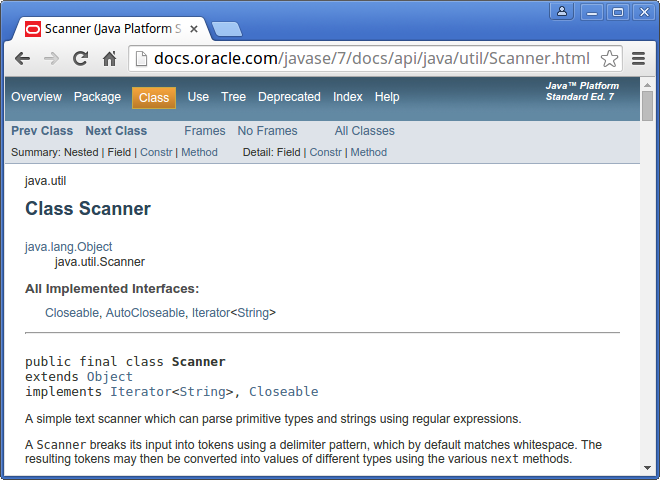
\includegraphics[width=\textwidth]{scanner.png}
\caption{Screenshot of the documentation for \java{Scanner} on Oracle's website.}
\end{figure}

Scroll down to the ``Method Summary'' section.
As you can see, the \java{Scanner} class provides quite a few methods.
In this chapter we'll focus on the ``next'' methods.
For example, click on the link for \java{nextInt}.

\begin{stdout}
public int nextInt()

Scans the next token of the input as an int.
\end{stdout}

\index{prototype}

The first line is the method's {\bf prototype}, which specifies the name of the method and its return type.
In this example, \java{nextInt} returns an \java{int}.
The next line describes what the method does.
The subsequent lines explain the parameters (if any) and return values.
The explanations are often redundant, but the documentation is supposed to fit this standard format.
%The last line describes the exceptions this method might throw.

It might take some time to get comfortable reading this kind of information, but it's well worth the effort.
Knowing what methods a class provides helps you avoid reinventing the wheel.
Whenever you learn about a new class, you should take a quick look at its documentation.
On that note, please take a few minutes and review the documentation for \java{System} and \java{String}.


\section{Floating-point numbers}

\index{floating-point}
\index{double (floating-point)}
\index{type!double}

In the last chapter we had some problems dealing with numbers that were not integers.
We worked around the problem by calculating percentages.
A more general solution is to use {\bf floating-point} numbers, which can represent fractions as well as integers.
As the name implies, the decimal point floats around (i.e., you can have as many decimal places as you want).

In Java, the default floating-point type is called \java{double}, which is short for double-precision.
You can create \java{double} variables and assign values to them using the same syntax we used for the other types:

\begin{code}
    double pi = 3.14159;
\end{code}

Although floating-point numbers are useful, they are a source of confusion because (1) there is an overlap between integers and doubles, and (2) computer hardware can only approximate real numbers.
Let's discuss these issues in more detail.

\subsection{Auto conversion}

%If you have the value {\tt 1}, is that an integer, a floating-point number, or both?

Java distinguishes the integer value {\tt 1} from the floating-point value {\tt 1.0}, even though they seem to be the same number.
They belong to different data types, and strictly speaking, you are not allowed to make assignments between types.

For example, the following is illegal because the variable on the left is an \java{int} and the value on the right is a \java{double}.

\begin{code}
    int x = 1.1;  // syntax error
\end{code}

It is easy to forget this rule, especially because there are situations where Java will {\em automatically} convert from one type to another.

\begin{code}
    double y = 1;  // bad style
\end{code}

The above example should be illegal, but Java allows it by converting the \java{int} to a \java{double} automatically.
This leniency is convenient, but it often causes problems for beginners. For example:

\begin{code}
    double y = 1 / 3;  // logic error
\end{code}

You might expect the variable {\tt y} to get the value {\tt 0.333333}, which is a legal floating-point value.
But instead it gets the value {\tt 0.0}.
The reason is that the expression on the right divides two integers.
So Java does {\em integer} division, which yields the value {\tt 0}.
Converted to \java{double}, the final result is {\tt 0.0}.

One way to solve this problem (after you finally discover that bug) is to make the right-hand side a floating-point expression. The following initializes {\tt y} to {\tt 0.333333}, as expected:

\begin{code}
    double y = 1.0 / 3.0;  // correct
\end{code}

\subsection{Rounding errors}

\index{arithmetic!floating-point}

The operations we have seen so far---addition, subtraction, multiplication, and division---also work on floating-point values, although you might be interested to know that the underlying mechanism is completely different.
In fact, most processors have special circuitry just for performing floating-point operations.

However there is a fundamental flaw with floating-point arithmetic.
In math, there are an infinite number of real numbers.
But computer processors are finite; they cannot represent {\em every} possible floating-point number.
Even with double-precision, you will frequently run into problems.

\begin{code}
    System.out.println(0.1 * 10);
    System.out.println(0.1 + 0.1 + 0.1 + 0.1 + 0.1
                     + 0.1 + 0.1 + 0.1 + 0.1 + 0.1);
\end{code}

On some machines, the output for the above example will be:

\begin{stdout}
    1.0
    0.9999999999999999
\end{stdout}

The problem here is that intermediate values may be rounded by the hardware.
Just remember that \java{double} values are always an approximation.


\section{Type casting}
\label{rounding}

Java converts an \java{int} to a \java{double} automatically, since no information is lost in the process.
On the other hand, going from \java{double} to \java{int} gets rid of the decimal places.
Java doesn't perform this operation automatically in order to ensure that you are aware of the loss of the fractional part of the number.

\index{type cast}

The simplest way to convert a floating-point value to an integer is to use a {\bf type cast}.
This operation is so called because it takes a value that belongs to one type and ``casts'' it into another type, in the sense of molding or reshaping the data.
The syntax for type casting is to put the name of the type in parentheses and use it as an operator.

\begin{code}
    double pi = 3.14159;
    int x = (int) pi;
\end{code}

\index{truncate}

The \java{(int)} operator has the effect of converting what follows into an integer.
In this example, \java{x} gets the value 3.
Converting to an integer always {\bf truncates} or rounds down, even if the fraction part is 0.99999999.

Type casting takes precedence over arithmetic operations.
In the following example, the value of \java{pi} gets converted to an integer first, and the result is 60.0, not 62.

\begin{code}
    double pi = 3.14159;
    double x = (int) pi * 20.0;
\end{code}

Operator precedence and integer truncation make type casting error-prone.
We will learn in the next chapter how to round floating-point numbers in the traditional way (i.e., to the closest integer).


\section{Formatting output}

When printing floating-point numbers, Java automatically decides how many decimal places to display.

\begin{code}
    System.out.print(7.0 / 3.0);
    // prints 2.3333333333333335   note: 5 is a rounding error
\end{code}

You can use \java{System.out.printf} to limit (or format) the number of decimal places. For example:

\begin{code}
    System.out.printf("%.3f", 7.0 / 3.0);
    // prints 2.333
\end{code}

The \java{printf} method takes two or more parameters, separated by commas.
Instead of just printing what is between the parentheses, \java{printf} allows for substitutions and formatting of output.
The first parameter is a {\em formatting string}.
It contains the text that you want to use, as well as positions where it will substitute other values.

\begin{code}
System.out.printf("The value is %.3f, okay?\n", value);
\end{code}

TODO


\section{Putting it all together}

TODO


\section{Testing via the command line}

TODO


\section{Formal languages}

\index{natural language}
\index{language!natural}

Learning a programming language is very different from learning a {\bf natural language} such as English, Spanish, French, or German.
The languages that people speak evolved naturally over time.
They were not designed by people, although we try to impose order on them for practical reasons.

\index{formal language}
\index{language!formal}

In contrast, {\bf formal languages} are designed by people for specific applications.
For example, the notation that mathematicians use is a formal language that is particularly good at denoting relationships among numbers and symbols.
Chemists use a formal language to represent the chemical structure of molecules.
And most importantly:

\index{programming language}
\index{language!programming}

\begin{quote}
{\bf Programming languages are formal languages that have been designed to express computations.}
\end{quote}

\index{syntax}
\index{semantics}

Formal languages have strict rules about both the {\bf syntax} (structure) and the {\bf semantics} (meaning) of statements.
For example, $3 + 3 = 6$ is a syntactically correct mathematical statement, but $3\ + = 3\ \$\ 6$ is not.
$1 + 2 = 4$ uses correct syntax, but is semantically incorrect.
$H_2O$ is a syntactically correct chemical formula, but $_2Zz$ is not.

\subsection{Tokens and grammar}

\index{token}

Syntax rules come in two flavors, pertaining to tokens and grammar.
{\bf Tokens} are the basic elements of the language, like words, numbers, and chemical elements.
One of the problems with $3\ + = 3\ \$\ 6$ is that $\$$ is not a legal token in mathematics.
Similarly, $_2Zz$ is not legal because there is no element with the abbreviation $Zz$.

\index{grammar}

The second type of syntax rule pertains to the {\bf grammar} of the language, or the way that individual tokens can be arranged.
The statement $3\ + = 3$ is structurally illegal, even though $+$ and $=$ are legal tokens, because you can't have one right after the other.
Similarly, in a chemical formula the subscript comes after the element name, not before.

\index{parse}

When you read a sentence in English or a statement in a formal language, you have to figure out the structure of the sentence (although in a natural language you do this unconsciously).
This process is called {\bf parsing}.
For example, when you hear the statement ``the penny dropped,'' you understand that the penny is the subject and dropped is the predicate.
After you have parsed the statement, you can begin to figure out what it means.
%Assuming that you know what a penny is and what it means to drop, you will understand the general implication of this statement.

Although formal and natural languages have features in common---tokens, grammar, and meaning---there are some differences.

\begin{description}

\term{ambiguity}
Natural languages are full of ambiguity, which people deal with by using contextual clues and other information.
Formal languages are designed to be nearly or completely unambiguous, which means that any statement has exactly one meaning, regardless of context.

\term{redundancy}
In order to make up for ambiguity and reduce misunderstandings, natural languages employ lots of redundancy.
As a result, they are often verbose.
Formal languages are less redundant and more concise.

\term{literalness}
Natural languages are full of idiom and metaphor.
When someone says ``the penny dropped'' there is no penny and nothing dropping.
This idiom means that someone finally realized something after a period of confusion.
In contrast, formal languages mean exactly what they say.

\end{description}

\subsection{Reading source code}

People who grow up speaking a natural language---that is, everyone---often have a hard time adjusting to formal languages.
In some ways, the difference between natural and formal language is like the difference between poetry and prose, but more so.

\begin{description}

\term{poetry}
Words are used for their sounds as well as for their meaning, and the whole poem together creates an effect or emotional response.
Ambiguity is not only common but often deliberate.

\term{prose}
The literal meaning of words is more important, and the structure contributes more meaning.
Prose is more amenable to analysis than poetry but still often ambiguous.

\term{program}
The meaning of a computer program is unambiguous and literal, and can be understood entirely by analysis of the tokens and grammar.

\end{description}

Here are some suggestions for reading programs (and other formal languages).
First, remember that formal languages are much more dense than natural languages, so it takes longer to read them.
Second, the structure is very important, so it is not always a good idea to read from top to bottom, left to right.
Over time you will learn to parse the program in your head, identifying the tokens and interpreting the structure.
Finally, the details matter.
Small errors in spelling and punctuation, which you can get away with in natural languages, can make a big difference in a formal language.
